\section{模型建立与求解}
\subsection{单通道确定性模型}
\subsubsection{模型建立}
\par 将校门前的道路网格化,假设行人占据一个网格、自行车占据两个网格。
根据假设,自行车在通过校门的时候会下车推行,
从而行人和自行车在门前的前进速度可以认为相同,设为$1m/s$。
对排队人群进行离散模拟,在每个模拟时间段内,如果行人或自行车前方空格
没有被占用,则前进一格。根据这样的模拟规则,将一个网格的长度设为$1m$。
\par 考虑单通行道的情况,模型可视化展示在图\ref{fig:1-lane-model}中。
\begin{figure}[ht]
    \centering
    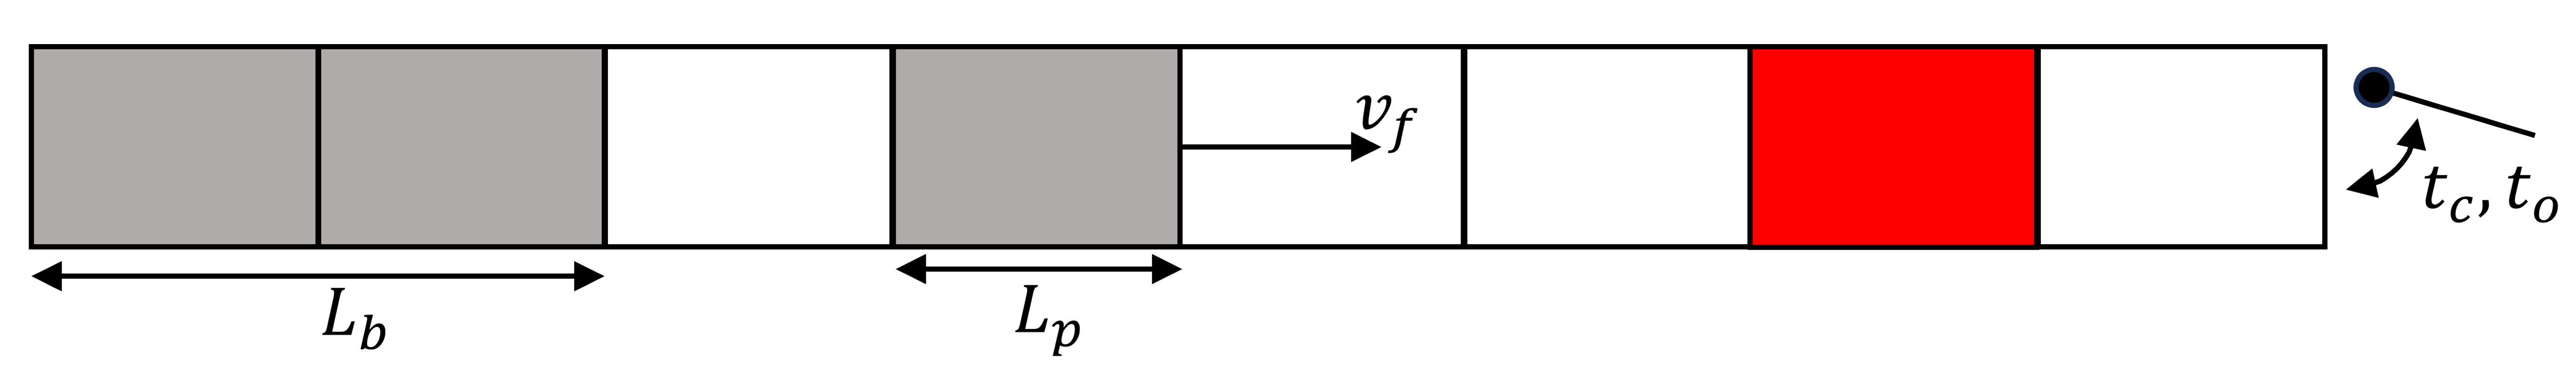
\includegraphics[width=0.6\textwidth]{images/cellular_automata_1_lane.png}
    \caption{单通行道模型可视化,其中灰色块表示网格被占用,红色块表示
    该通行者会刷卡失败(或没有校园卡),图中最右部分为校门}
    \label{fig:1-lane-model}
\end{figure}
\newline 其中:
\begin{itemize}
    \item $L_p, L_b$分别表示行人和自行车占用的网格长度
    \item $v_f$表示行人和自行车的前进速度
    \item $t_o, t_c$分别表示校门的开关时间,考虑实际情况,认为$t_c=t_o$
    \item $t_g,t_p$(图中未标注)分别为刷卡时间和通过时间,在确定性模型中
    两者视为定值
\end{itemize}
人和自行车均在道路最左边生成,道路有最大长度,当道路最左侧已经被占用时,
不再生成人。认为人的生成过程是一个泊松过程,对于高人流量和低人流量的时间段
泊松过程的参数取值不同。
\par 刷卡进校过程的拆分及两种开门方式的不同展示在图\ref{fig:process-entering-gate}中。
\begin{figure}[ht]    
    \centering
    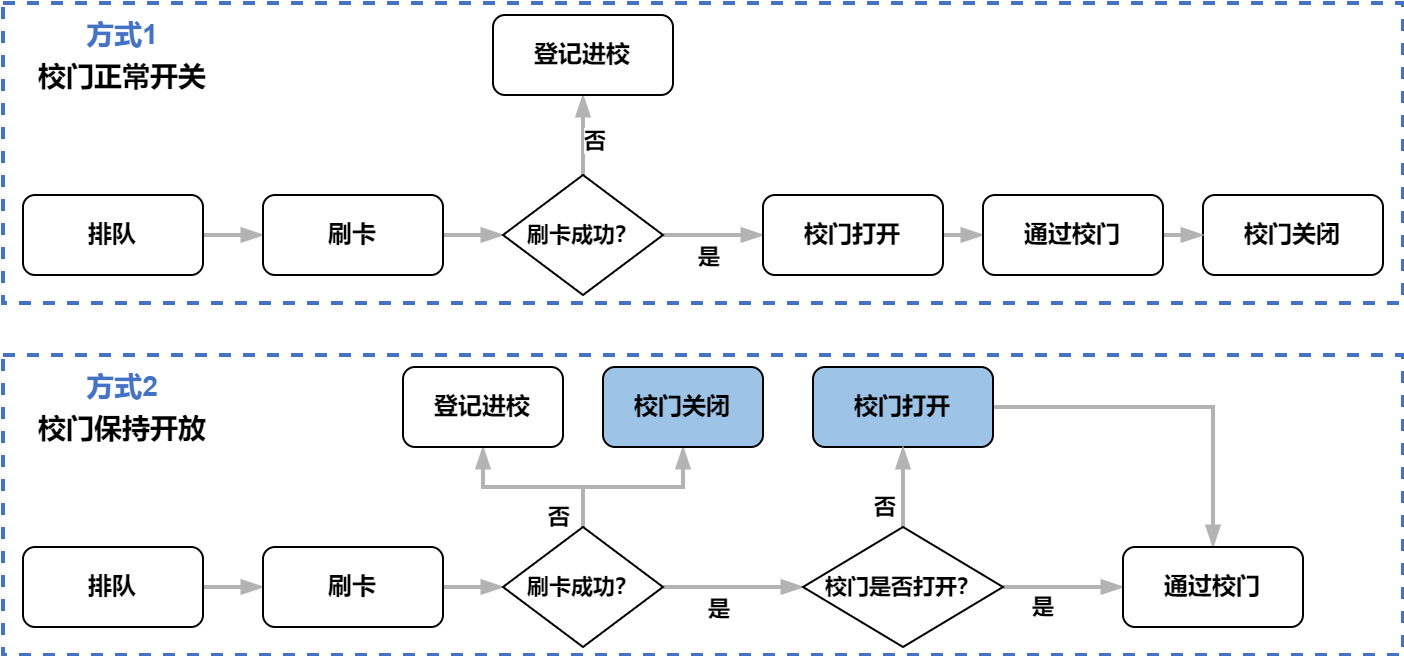
\includegraphics[width=.7\textwidth]{images/enter_gate_process.png}
    \caption{刷卡进校过程及两种校门开关方式的异同}
    \label{fig:process-entering-gate}
\end{figure}
在刷卡进校时,对于两种方法做相应的时间消耗分析:
\begin{itemize}
    \item 门保持开放:
    \begin{itemize}
        \item 如果刷卡成功,直接通过校门,需要的时间即为通过校门的时间加上
        刷卡识别的时间$t_p+t_g$。如果上一个人刷卡失败,该时间变为$t_g+t_o+t_p$。
        \item 如果刷卡失败,需要等待门关闭。根据实际生活经验,刷卡失败
        的个体在刷卡过程中一般花费时间也较长(例如询问在哪里刷身份证),同时
        刷卡失败之后,一般要离开队伍,然后登记入校。
        将这两个过程中时间的消耗合计为
        $t_{penal}$,从而刷卡失败消耗的时间为刷卡时间、等待门关闭的时间和
        离开队伍的时间加和$t_g+t_c+t_{penal}$。
    \end{itemize}
    \item 门正常开关:
    \begin{itemize}
        \item 如果刷卡成功,等待门开放后通过校门,下一个在队伍中的人等待门
        关闭后继续刷卡通过。从而一个人需要的时间为$t_g+t_o+t_p+t_c$。
        \item 如果刷卡失败,需要离开队伍。门正常开关时,不用等待门关闭,
        从而所需时间为$t_g+t_{penal}$。
    \end{itemize}
\end{itemize}

\subsubsection{数值模拟}
模拟的时间步长$t^*$取为$0.5s$,根据实际生活经验,约定开门的时间$t_o=t^*$、
行人的刷卡时间$t_g=t^*$、通过时间$t_p=t^*$、门关上的时间$t_c=t_o=t^*$。
如果刷卡失败,耽误的时间$t_{penal}=2t^*$。根据模型分析:
\begin{itemize}
    \item 门保持开放:
    \begin{itemize}
        \item 刷卡成功:耗时$t_p+t_g=2t^*$。
        \item 刷卡失败:耗时$t_g+t_c+t_{penal}=4t^*$。
    \end{itemize}
    \item 门正常开关:
    \begin{itemize}
        \item 刷卡成功:耗时$t_g+t_o+t_p+t_c=4t^*$。
        \item 刷卡失败:耗时$t_g+t_{penal}=3t^*$
    \end{itemize}
\end{itemize}

\subsection{单通道随机性模型}
\subsubsection{模型建立}
在确定性模型中,刷卡时间和通行时间(之后统称为服务时间)认为是常数,
在实际情况中,服务时间往往会因为客户对象的不同而发生变化\footnote{
    例如,由于老年人的刷卡时间和通过时间相较年轻人明显较长,
    所以老年人的服务时间将会明显长于年轻人。
}。选择利用负指数分布刻画这种服务时间的不确定性,从而更好地刻画队伍的运动情况。


\subsection{多通道模型}
\par 实际情况中,往往有多条入校通道。相较于单通道,多通道的引入,使得
行人和自行车在条件允许时,可以选择更换通道,从而更快地通过校门。
在实际情况中,如果当前通道有人刷卡失败
